\subsection{Der Helmholtzspulen Versuch}
\fbox{
	\parbox{\linewidth}{
		\textit{Ziel des Kapitels:}\\
		Anwendungsfall und Hintergrund vorstellen.\\[6px]
		\textit{Inhalte:}
		\begin{itemize}
			\item Physikalischer Hintergrund
			\item Versuchsaufbau und Ablauf
		\end{itemize}
		
		\textit{Wichtige Literatur:}	
		\begin{itemize}
			\item TODO Beschreibung zu Verusch aus Buch angeben
		\end{itemize}
}}

Helmholtz-Spulen werden in der Physik an verschiedensten Stellen verwendet und spielen auch in der Ausbildung von Schülern und Studenten eine wichtige Rolle. Unter anderem werden sie in Schülerversuchen genutzt, um experimentell die Stärke des Erdmagnetfeldes zu bestimmen. Im Folgenden sollen die physikalischen Hintergründe kurz eingeführt sowie Versuchsaufbau und -Ablauf erläutert werden.

\subsubsection{Physikalischer Hintergrund}
Wird eine elektrische Leiterschleife von einem Strom durchflossen, so induziert diese ein Magnetfeld. Dieses Feld verläuft sowohl durch das Innere als auch durch die Umgebung der Spule. Die Stärke des Feldes hängt dabei von der Windungszahl und dem Durchmesser der Spule sowie der angelegten Spannung ab.
Im Inneren der Spule ist das Magnetfeld \textit{homogen}. Das bedeutet, es ist an allen Punkten im Raum gleich stark und gleich gerichtet. Außerhalb der Spule hingegen ist das Feld \textit{inhomogen}, es erfüllt beide zuvor genannten Eigenschaften nicht.\\

Bei einer Helmholtz-Spule handelt es sich im Prinzip um zum zwei zusammengeschaltete solcher Spulen. Dabei werden zwei identische Spulen nebeneinander aufgestellt und verbunden, sodass der Abstand genau dem Radius der Spulen entspricht. Abbildung \ref{img:Helmholtz} zeigt eine solche Helmholtz-Spule.\\

Durch diese spezielle Eigenschaft des Aufbaus überlagern sich die beiden, durch die einzelnen Spulen entstehenden Magnetfelder genau so, dass im Raum zwischen den Spulen ebenfalls ein homogenes Magnetfeld entsteht.
	
\begin{figure}[h!]
	\centering
	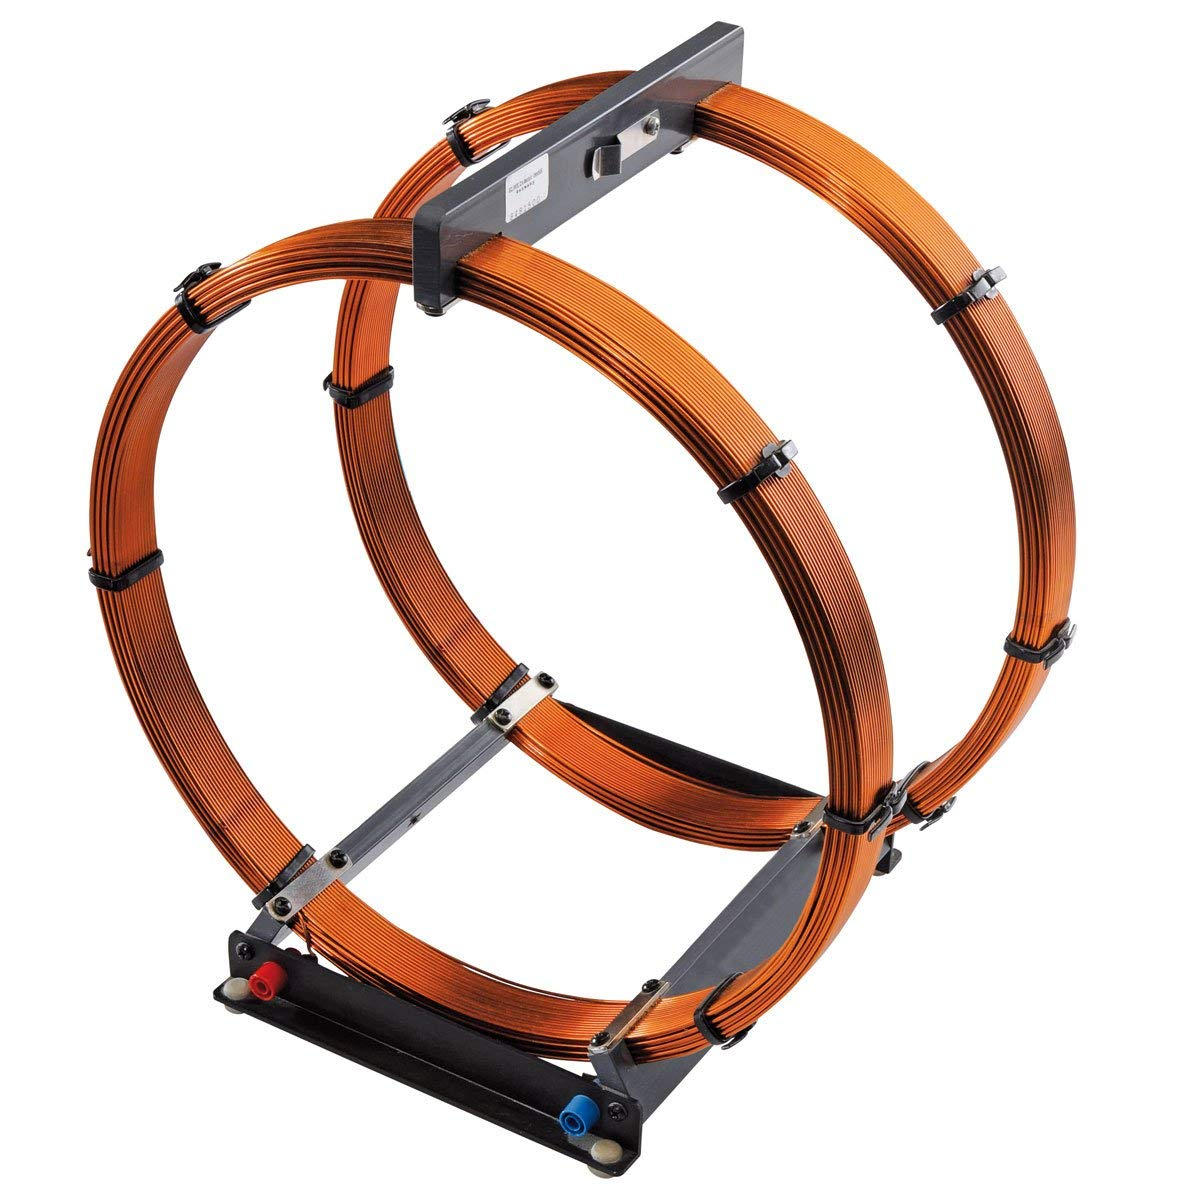
\includegraphics[width=1\textwidth]{images/Helmholtz.jpg}
	\caption{HH Spule}
	\label{img:Helmholtz}
\end{figure}

\begin{itemize}
	\item Homogenes Magnetfeld innerhalb Helmholtz-Spule
	\item Magnetfeld überlagerung, Vektoraddition
	\item Kompensation von Erdmagnetfeld
	\item ...
\end{itemize}

\subsubsection{Versuchsaufbau}
\begin{itemize}
	\item Helmholtz-Spulen, Windungszahl X, Abstand Y, Durchmesser Z
	\item Spannungsgenerator mit Spannung, Stromstärke, AC/DC
	\item Frei beweglicher Kompass im inneren der Spulen
	\item Rotation der Spulen sowie Spannungsanpassung durch Nutzer
	\item ... bis Kompass im inneren kein Magnetfeld mehr wahrnimmt
	\item ... dann ist das Magnetfeld der Erde genau kompensiert, d.h. genau so stark aber entgegengesetzt gerichtet zum Feld der Spulen
	\item Keine weitere Schutzausrüstung oder Messinstrumente notwendig
\end{itemize}